\chapter{Plannification et Organisation}

\section{Planning prévisionnel}

Pour mener à bien le projet ce semestre, nous avons établi un planning prévisionnel détaillé basé sur les contraintes académiques et les jalons de rendus. Ce diagramme présente la répartition temporelle des tâches pour l'ensemble du groupe.

\begin{figure}[H]
    \centering
    \begin{ganttchart}[
        vgrid,
        hgrid,
        x unit=1.2cm,
        y unit title=0.8cm,
        y unit chart=0.6cm,
        title label font=\scriptsize\bfseries,
        bar label font=\tiny,
        group label font=\scriptsize\bfseries,
        milestone label font=\tiny\itshape
    ]{6}{23}
    
    % --- Titres des colonnes (Semaines) ---
    \gantttitle{Semaines du Semestre (S6 à S23)}{18} \\
    \gantttitlelist{6,...,23}{1} \\

    % --- SECTION 1 : GESTION & RENDUS ---
    \ganttgroup{Jalons \& Rendus}{6}{23} \\
    \ganttbar{Répartition des tâches}{6}{9} \\
    \ganttmilestone[milestone/.append style={fill=red}]{Rapport 1 (02/03)}{10} \\
    \ganttmilestone[milestone/.append style={fill=red}]{Rapport 2 (27/04)}{18} \\
    \ganttmilestone[milestone/.append style={fill=red}]{Rapport Final (05/06)}{23} \\

    % --- SECTION 2 : TACHES TECHNIQUES ---
    \ganttgroup{Node Red Solution (Rudy, Amandine)}{10}{22} \\
    \ganttbar{Développement solution}{10}{17} \\
    \ganttbar{Tests de communication}{19}{22} \\
    
    \ganttgroup{Alimentations \& Tests (?)}{6}{22} \\
    \ganttbar{Analyse \& CdC détaillé (?) }{6}{9} \\
    \ganttbar{Simulations, Schémas, PCB (?) }{10}{17} \\
    \ganttbar{Commande composants (?) }{12}{14} \\
    \ganttbar{Réalisation montage \& Validation (?) }{19}{22} \\

    % --- SECTION 3 : PERIODES SPECIALES ---
    \ganttbar[bar/.append style={fill=gray!30}]{Vacances / Examens}{16}{17}

    % Liens (dépendances simplifiées)
    \ganttlink{elem1}{elem2} 
    \ganttlink{elem2}{elem5} 
    
    \end{ganttchart}
    \caption{Diagramme de Gantt prévisionnel du projet S8}
    \label{fig:gantt_projet}
\end{figure}

\section{Organisation de l'équipe}
L'organisation de l'équipe pour ce semestre est présentée ci-dessous :
\begin{figure}[H]
    \centering
    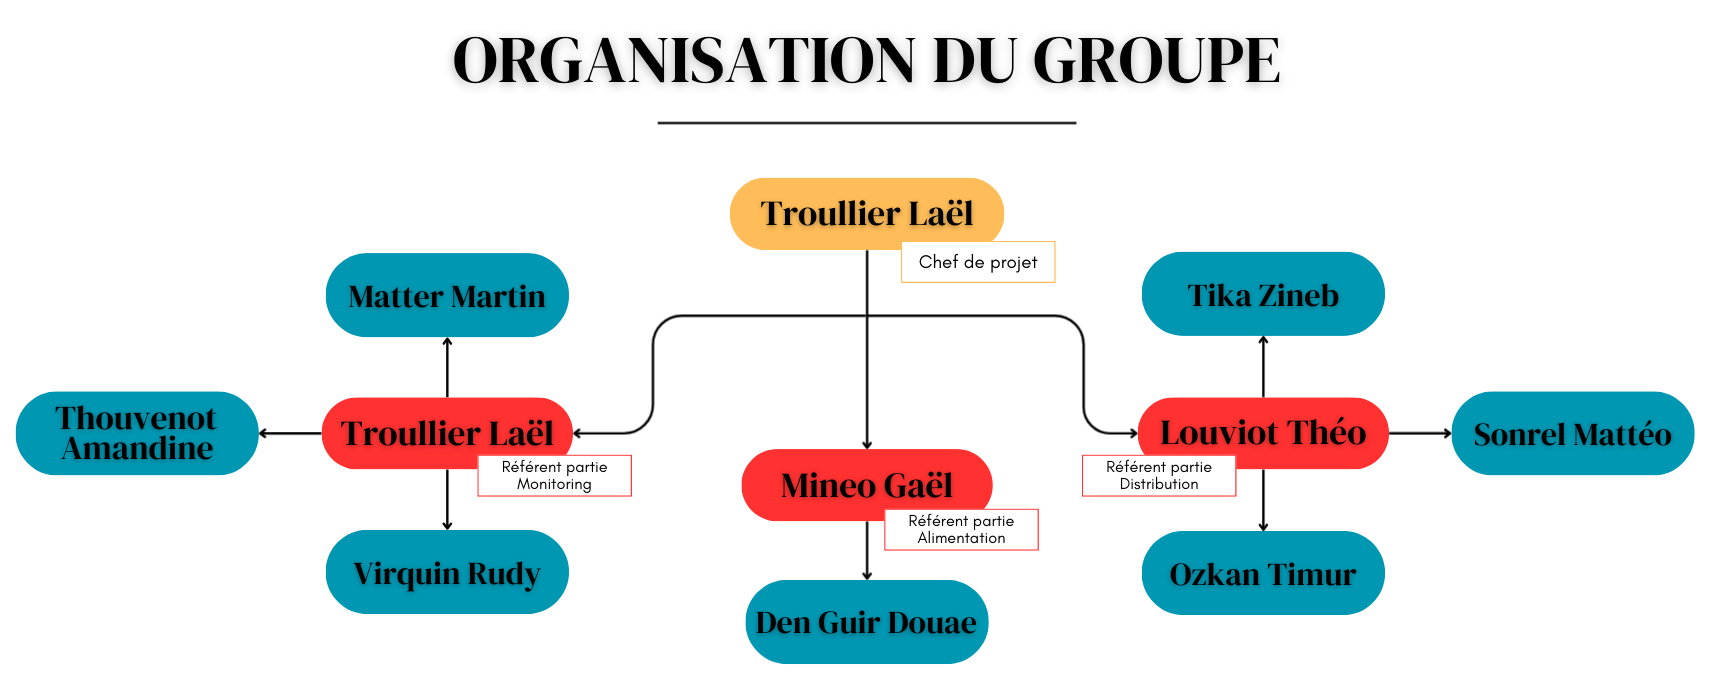
\includegraphics[width=1\textwidth]{images/diagrammes/Organigramme Projet S8.png}
    \caption{Organigramme du Projet S8}
    \label{fig:organigramme}
\end{figure}